\documentclass[a4paper, 12pt]{article}
\usepackage{graphicx}
\usepackage[utf8]{inputenc}
\usepackage[ukrainian]{babel}
\usepackage{amsmath}
\usepackage{fancyhdr}
\usepackage{geometry}
\geometry{top=2cm, bottom=2cm, left=3cm, right=1.5cm}
\usepackage[colorlinks=true,linkcolor=blue]{hyperref}%
\begin{document}

\begin{titlepage}
	\begin{center}
		\Large
		\textbf{Київський національний університет імені Тараса Шевченка} \\
		Факультет комп'ютерних наук та кібернетики \\

		\vspace{6cm}

		\textbf{\LARGE ЗВІТ ДО ЛАБОРАТОРНОЇ РОБОТИ №2} \\[0.5cm]
		\textbf{З дисципліни ``Чисельні методи''} \\[0.5cm]
		\textbf{Тема: Розв'язування системи лінійних алгебраїчних рівнянь} \\

		\vfill
		\hspace{7cm} Виконав студент 3-го курсу \\
		\hspace{7cm} групи ТТП-31 \\
		\hspace{7cm} Рісенгін Владислав \\
		\vspace{2cm}

		Київ-2024
	\end{center}
\end{titlepage}

\newpage

\hbadness=99999

\section{Постановка задачі}

Варіант № 3. Метод Гаусса, метод прогонки, метод Зейделя.

Згенерувати матрицю 4х4 з цілими елементами за модулем менше 10 та вектор правої частини з урахуванням обмежень та достатніх умов збіжності, що накладаються методами у вашому варіанті. Порахувати визначник матриці та обернену матрицю тими методами, що мають відповідне застосування. Для ітераційного методу бажану точність розв’язку СЛАР зробити параметром, який може вводити користувач.

\section{Вступ}

Метою цієї лабораторної роботи є вивчення методів розв'язування системи лінійних алгебраїчних рівнянь, які дають можливість вирішення багатьох наукових та інженерних задач. У процесі виконання роботи будуть досліджені та реалізовані методи Гауса, прогонки, Зейделя.

\section{Деталі реалізації}

Лабораторна робота виконана використовуючи мову програмування Python, а також бібліотеку numpy.

\clearpage
\section{Теоретичний опис методів}
\subsection{Метод Гауса}

\begin{figure}[ht]
	\centering
	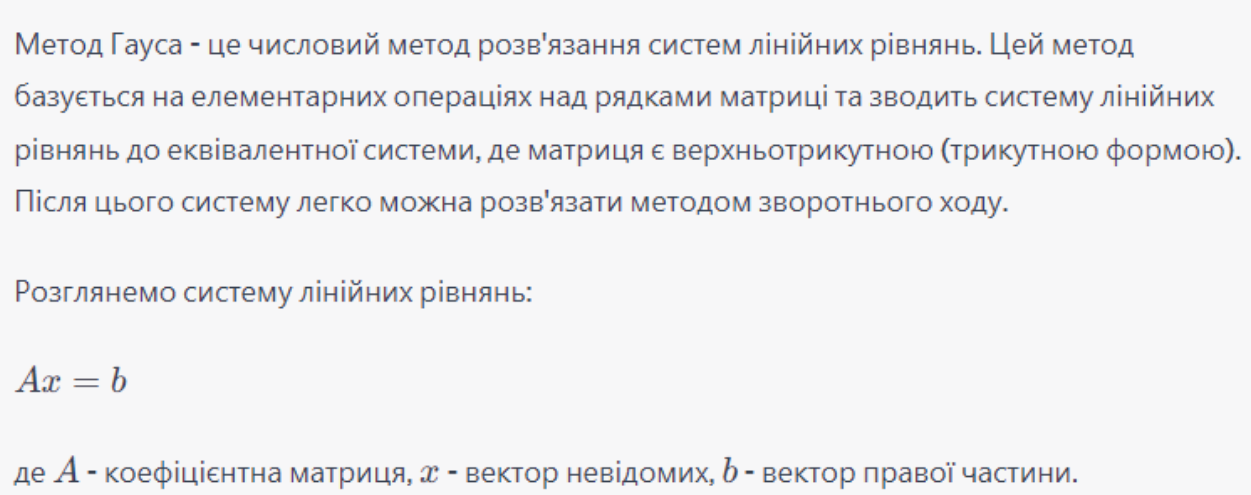
\includegraphics[width=0.75\linewidth]{gauss1.png}
\end{figure}
\begin{figure}[ht]
	\centering
	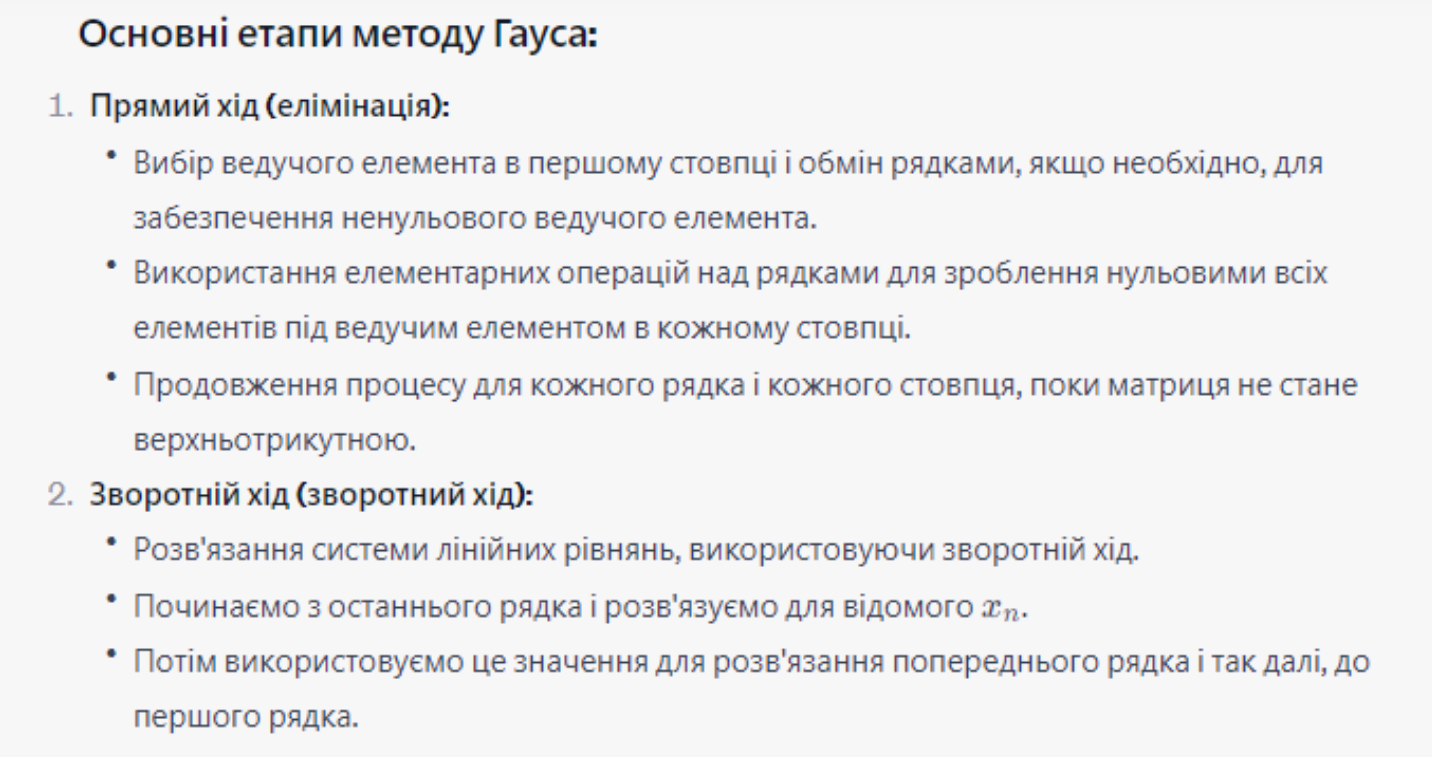
\includegraphics[width=0.75\linewidth]{gauss2.png}
\end{figure}
\begin{figure}[ht]
	\centering
	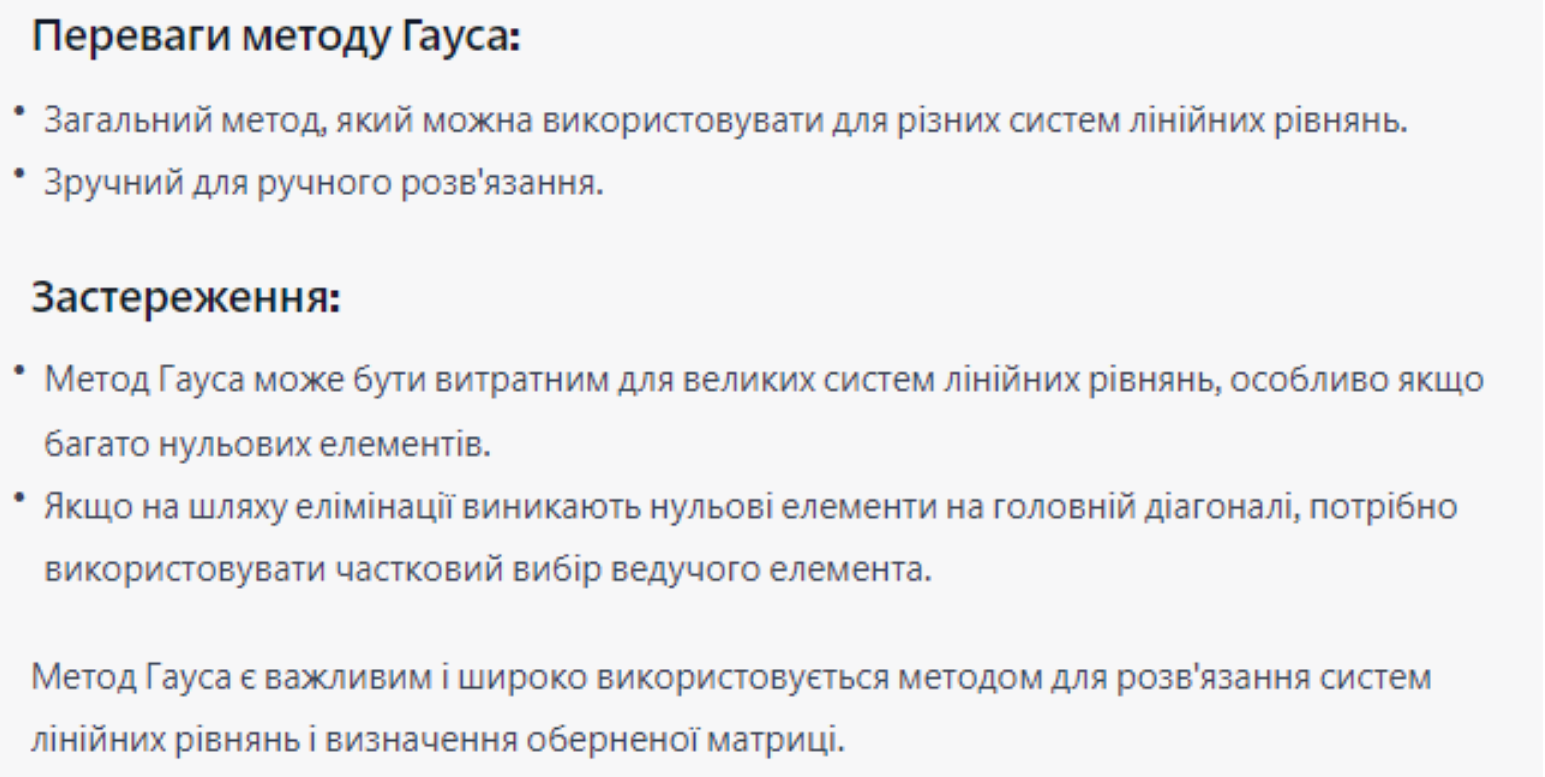
\includegraphics[width=0.75\linewidth]{gauss3.png}
\end{figure}

\clearpage
\newpage
\subsection{Метод прогонки (Томаса)}

\begin{figure}[ht]
	\centering
	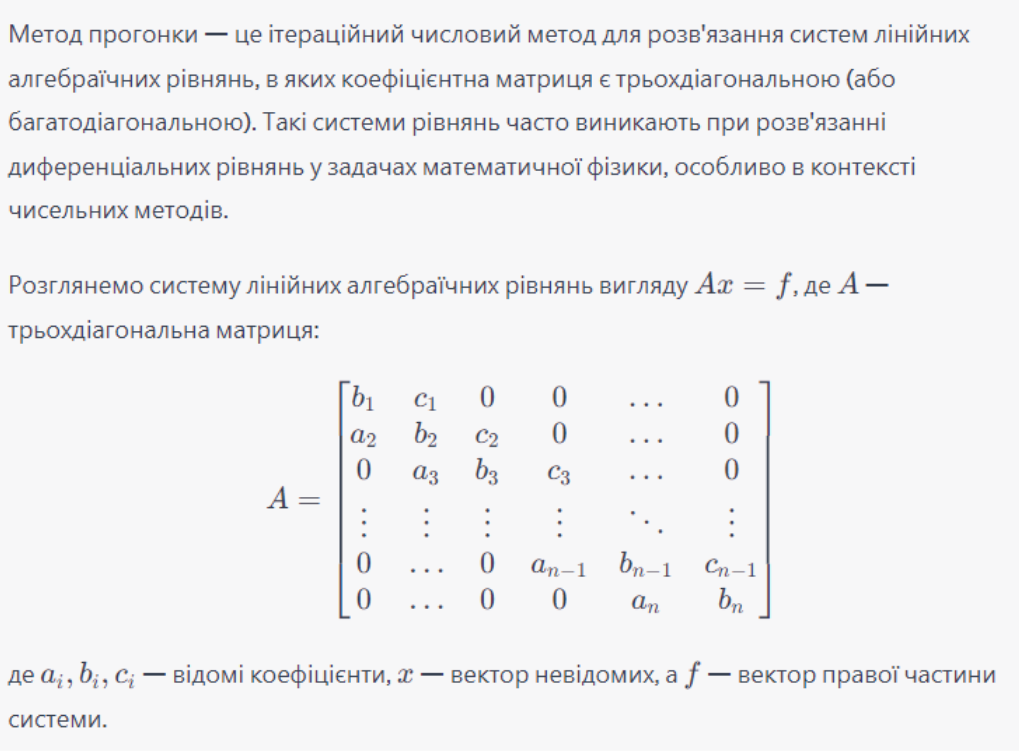
\includegraphics[width=0.75\linewidth]{progonka1.png}
\end{figure}
\begin{figure}[ht]
	\centering
	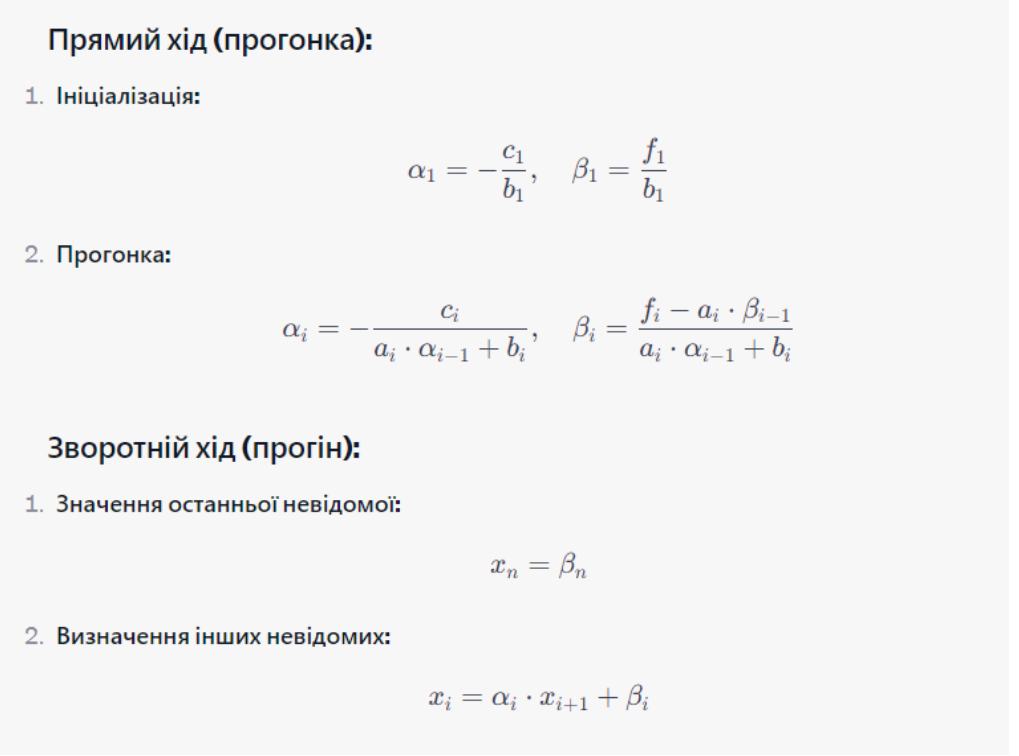
\includegraphics[width=0.75\linewidth]{progonka2.png}
\end{figure}
\begin{figure}[ht]
	\centering
	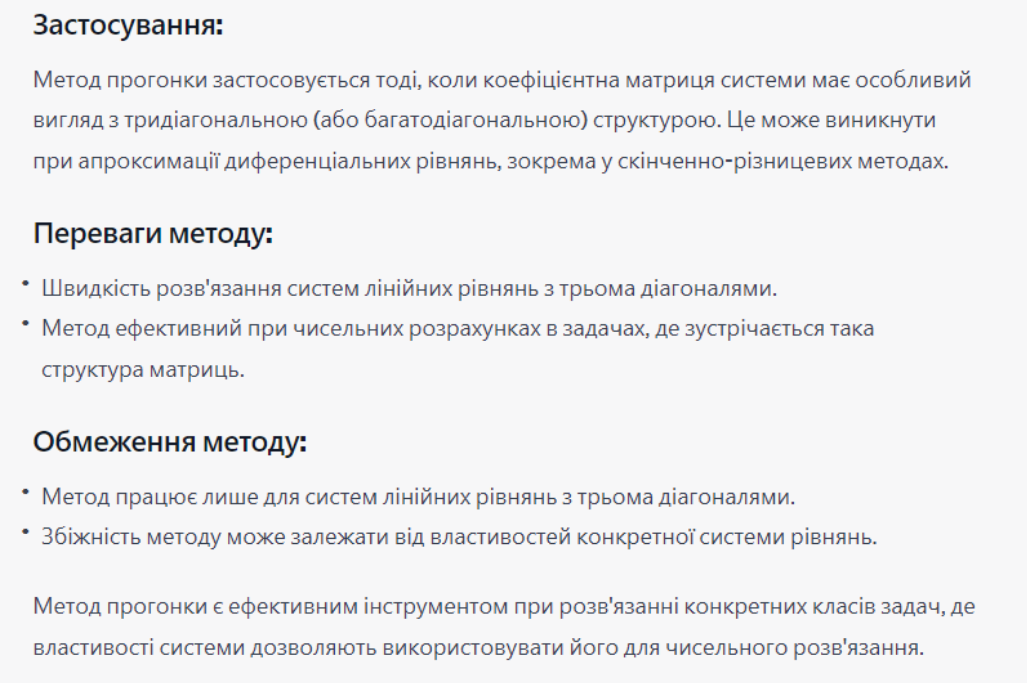
\includegraphics[width=0.75\linewidth]{progonka3.png}
\end{figure}

\clearpage
\newpage
\subsection{Метод Зейделя}

\begin{figure}[ht]
	\centering
	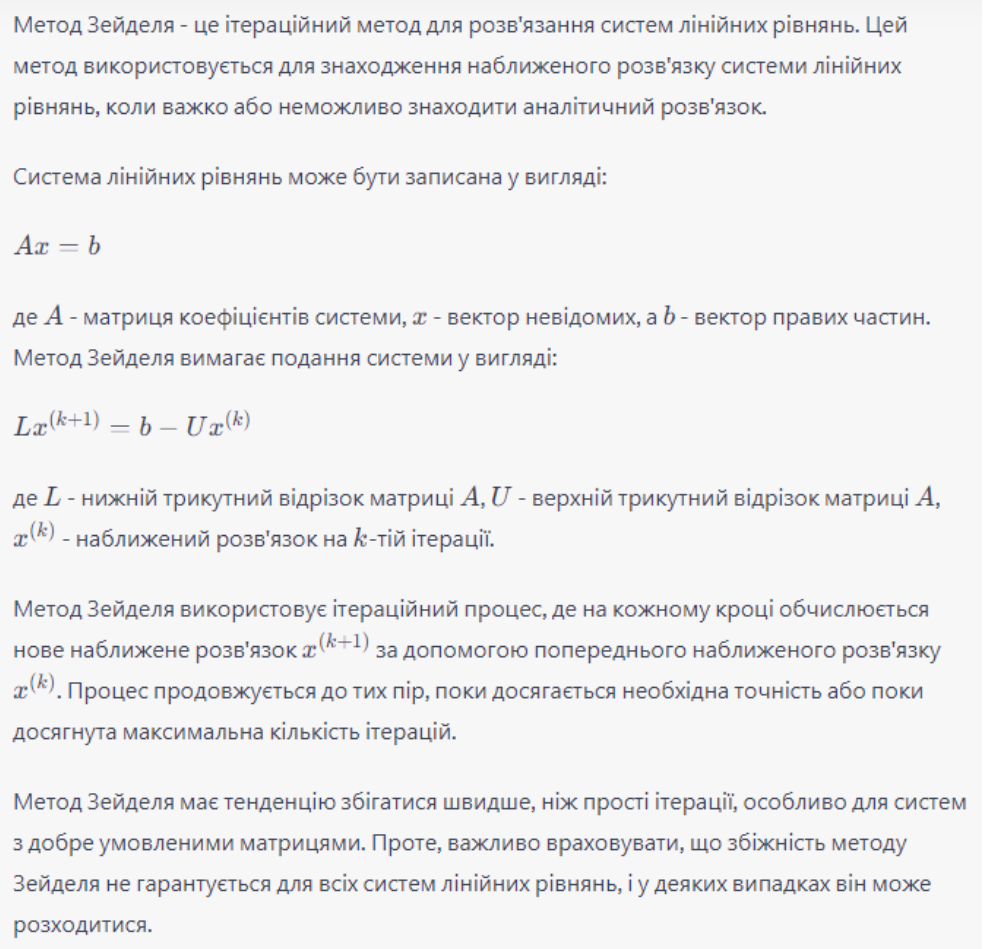
\includegraphics[width=0.8\linewidth]{seidel1.png}
\end{figure}
\begin{figure}[ht]
	\centering
	
\includegraphics[width=0.8\linewidth]{seidel2.png}
\end{figure}

\newpage
\section{Результати роботи програми}

\subsection{Метод Гауса}
Задача полягає в тому, щоб розв'язати систему лінійних алгебраїчних рівнянь методом Гауса. Використовуючи елементарні перетворення рядків, ми приводимо розширену матрицю до верхньої трикутної форми.

Початкова матриця системи:
\[
\[
\begin{bmatrix}
14 & 0 & 2 & 8 &\bigm| & 5 \\
0 & 30 & -3 & -9 &\bigm| & 9 \\
3 & -4 & 12 & 2 &\bigm| & -6 \\
-6 & 7 & -2 & 33 &\bigm| & 26 \\
\end{bmatrix}
\sim
\begin{bmatrix}
1 & 0 & 0.1429 & 0.5714 &\bigm| & 0.3571 \\
0 & 30 & -3 & -9 &\bigm| & 9 \\
3 & -4 & 12 & 2 &\bigm| & -6 \\
-6 & 7 & -2 & 33 &\bigm| & 26 \\
\end{bmatrix} 

\sim
\begin{bmatrix}
1 & 0 & 0.1429 & 0.5714 &\bigm| & 0.3571 \\
0 & 30 & -3 & -9 &\bigm| & 9 \\
0 & -4 & 11.5714 & 0.2857 &\bigm| & -7.0714 \\
-6 & 7 & -2 & 33 &\bigm| & 26 \\
\end{bmatrix}
\sim
\begin{bmatrix}
1 & 0 & 0.1429 & 0.5714 &\bigm| & 0.3571 \\
0 & 30 & -3 & -9 &\bigm| & 9 \\
0 & -4 & 11.5714 & 0.2857 &\bigm| & -7.0714 \\
0 & 7 & -1.1429 & 36.4286 &\bigm| & 28.1429 \\
\end{bmatrix}
\]

\sim
\[
\begin{bmatrix}
1 & 0 & 0.1429 & 0.5714 &\bigm| & 0.3571 \\
0 & 1 & -0.1 & -0.3 &\bigm| & 0.3 \\
0 & 0 & 11.1714 & -0.9143 &\bigm| & -5.8714 \\
0 & 0 & -0.4429 & 38.5286 &\bigm| & 26.0429 \\
\end{bmatrix}
\sim
\begin{bmatrix}
1 & 0 & 0.1429 & 0.5714 &\bigm| & 0.3571 \\
0 & 1 & -0.1 & -0.3 &\bigm| & 0.3 \\
0 & 0 & 1 & -0.0818 &\bigm| & -0.5256 \\
0 & 0 & 0 & 38.4923 &\bigm| & 25.8101 \\
\end{bmatrix}


\sim
\begin{bmatrix}
1 & 0 & 0.1429 & 0.5714 &\bigm| & 0.3571 \\
0 & 1 & -0.1 & -0.3 &\bigm| & 0.3 \\
0 & 0 & 1 & -0.0818 &\bigm| & -0.5256 \\
0 & 0 & 0 & 1 &\bigm| & 0.6705 \\
\end{bmatrix}
\]
\sim
\[
\begin{bmatrix}
1 & 0 & 0.1429 & 0 &\bigm| & -0.0260 \\
0 & 1 & -0.1 & 0 &\bigm| & 0.4541 \\
0 & 0 & 1 & 0 &\bigm| & -0.4707 \\
0 & 0 & 0 & 1 &\bigm| & 0.6705 \\
\end{bmatrix}

\sim
\begin{bmatrix}
1 & 0 & 0 & 0 &\bigm| & 0.0412 \\
0 & 1 & 0 & 0 &\bigm| & 0.4541 \\
0 & 0 & 1 & 0 &\bigm| & -0.4707 \\
0 & 0 & 0 & 1 &\bigm| & 0.6705 \\
\end{bmatrix}
\]

\textbf{Final solution:} \\
\mathbf{x} = [ 0.04122787  0.4540879  -0.47069865  0.6705259 ]

Перевіримо розв'язок \((x_1, x_2, x_3, x_4) = (0.0412, 0.4541, -0.4707, 0.6705)\) підставивиши у початкове рівняння: \[ \begin{aligned} 14 \cdot x_1 + 0 \cdot x_2 + 2 \cdot x_3 + 8 \cdot x_4 &= 5 \\ 0 \cdot x_1 + 30 \cdot x_2 - 3 \cdot x_3 - 9 \cdot x_4 &= 9 \\ 3 \cdot x_1 - 4 \cdot x_2 + 12 \cdot x_3 + 2 \cdot x_4 &= -6 \\ -6 \cdot x_1 + 7 \cdot x_2 - 2 \cdot x_3 + 33 \cdot x_4 &= 26 \\ \end{aligned} \] \[ \begin{aligned} 14 \cdot 0.0412 + 0 \cdot 0.4541 + 2 \cdot (-0.4707) + 8 \cdot 0.6705 &= 5 \quad (5 = 5) \\ 0 \cdot 0.0412 + 30 \cdot 0.4541 - 3 \cdot (-0.4707) - 9 \cdot 0.6705 &= 9 \quad (9 = 9) \\ 3 \cdot 0.0412 - 4 \cdot 0.4541 + 12 \cdot (-0.4707) + 2 \cdot 0.6705 &= -6 \quad (-6 = -6) \\ -6 \cdot 0.0412 + 7 \cdot 0.4541 - 2 \cdot (-0.4707) + 33 \cdot 0.6705 &= 26 \quad (26 = 26) \\ \end{aligned} \] Отже, розв'язок задовольняє початковим умовам.
\clearpage
\subsection{Метод прогонки}

\begin{center}
\begin{bmatrix}
11 & 8 & 0 & 0 &\bigm| & 7 \\ 
2 & 3 & 0 & 0 &\bigm| & 12 \\
0 & 0 & 9 & -8 &\bigm| & 22 \\
0 & 0 & 2 & 3 &\bigm| & -19
\end{bmatrix}
\end{center}

Перевіримо діагональну перевагу для кожного рядка:

1. Для першого рядка:
   \[
   |11| > |8| + |0| + |0| \quad \Rightarrow \quad 11 > 8 + 0 + 0 \quad \Rightarrow \quad 11 > 8 \quad \text{(вірно)}
   \]

2. Для другого рядка:
   \[
   |3| > |2| + |0| + |0| \quad \Rightarrow \quad 3 > 2 + 0 + 0 \quad \Rightarrow \quad 3 > 2 \quad \text{(вірно)}
   \]

3. Для третього рядка:
   \[
   |9| > |0| + |0| + |-8| \quad \Rightarrow \quad 9 > 0 + 0 + 8 \quad \Rightarrow \quad 9 > 8 \quad \text{(вірно)}
   \]

4. Для четвертого рядка:
   \[
   |3| > |0| + |0| + |2| \quad \Rightarrow \quad 3 > 0 + 0 + 2 \quad \Rightarrow \quad 3 > 2 \quad \text{(вірно)}


\begin{figure}[h]
	\centering
	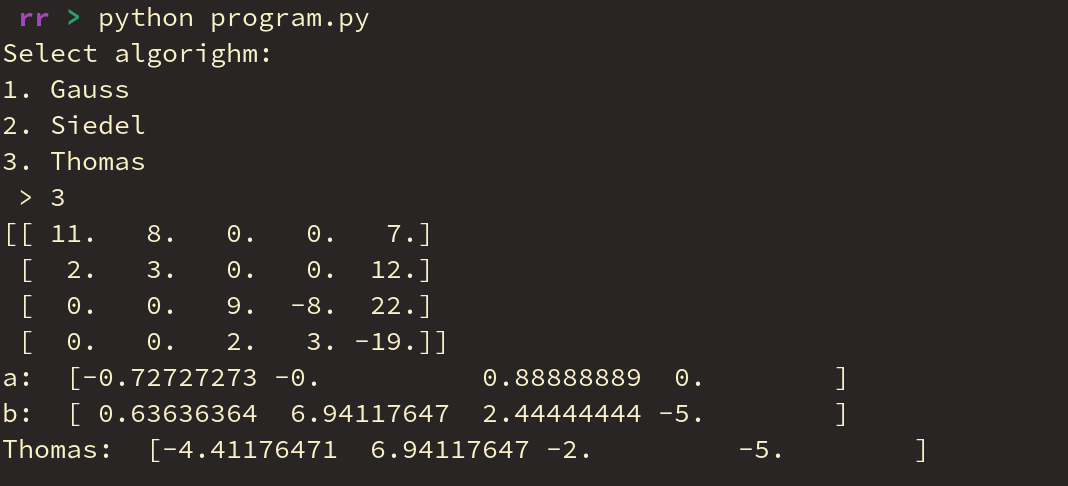
\includegraphics[width=0.8\linewidth]{thomas_result.png}
\end{figure}

Перевіримо розв'язок \((x_1, x_2, x_3, x_4) = (-4.4118, 6.9412, -2, -5)\), підставивши його у початкове рівняння:

\[
\begin{aligned}
    11 \cdot x_1 + 8 \cdot x_2 + 0 \cdot x_3 + 0 \cdot x_4 &= 7 \\
    2 \cdot x_1 + 3 \cdot x_2 + 0 \cdot x_3 + 0 \cdot x_4 &= 12 \\
    0 \cdot x_1 + 0 \cdot x_2 + 9 \cdot x_3 - 8 \cdot x_4 &= 22 \\
    0 \cdot x_1 + 0 \cdot x_2 + 2 \cdot x_3 + 3 \cdot x_4 &= -19 \\
\end{aligned}
\]

Підставляємо значення \(x_1 = -4.4118\), \(x_2 = 6.9412\), \(x_3 = -2\), \(x_4 = -5\):

\[
\begin{aligned}
    11 \cdot (-4.4118) + 8 \cdot 6.9412 + 0 \cdot (-2) + 0 \cdot (-5) &= 7 \quad (7 = 7) \\
    2 \cdot (-4.4118) + 3 \cdot 6.9412 + 0 \cdot (-2) + 0 \cdot (-5) &= 12 \quad (12 = 12) \\
    0 \cdot (-4.4118) + 0 \cdot 6.9412 + 9 \cdot (-2) - 8 \cdot (-5) &= 22 \quad (22 = 22) \\
    0 \cdot (-4.4118) + 0 \cdot 6.9412 + 2 \cdot (-2) + 3 \cdot (-5) &= -19 \quad (-19 = -19) \\
\end{aligned}
\]

Розв'язок коректний.

\newpage
\subsection{Метод Зейделя}

Знайдемо розв'язок з точністю $\epsilon < 10^{-5}$ \\
Як критерій зупинки використовується норма $max(|x_1|, |x_2|, ..., |x_n|) < \epsilon$ \\ 

\begin{figure}[h]
	\centering
	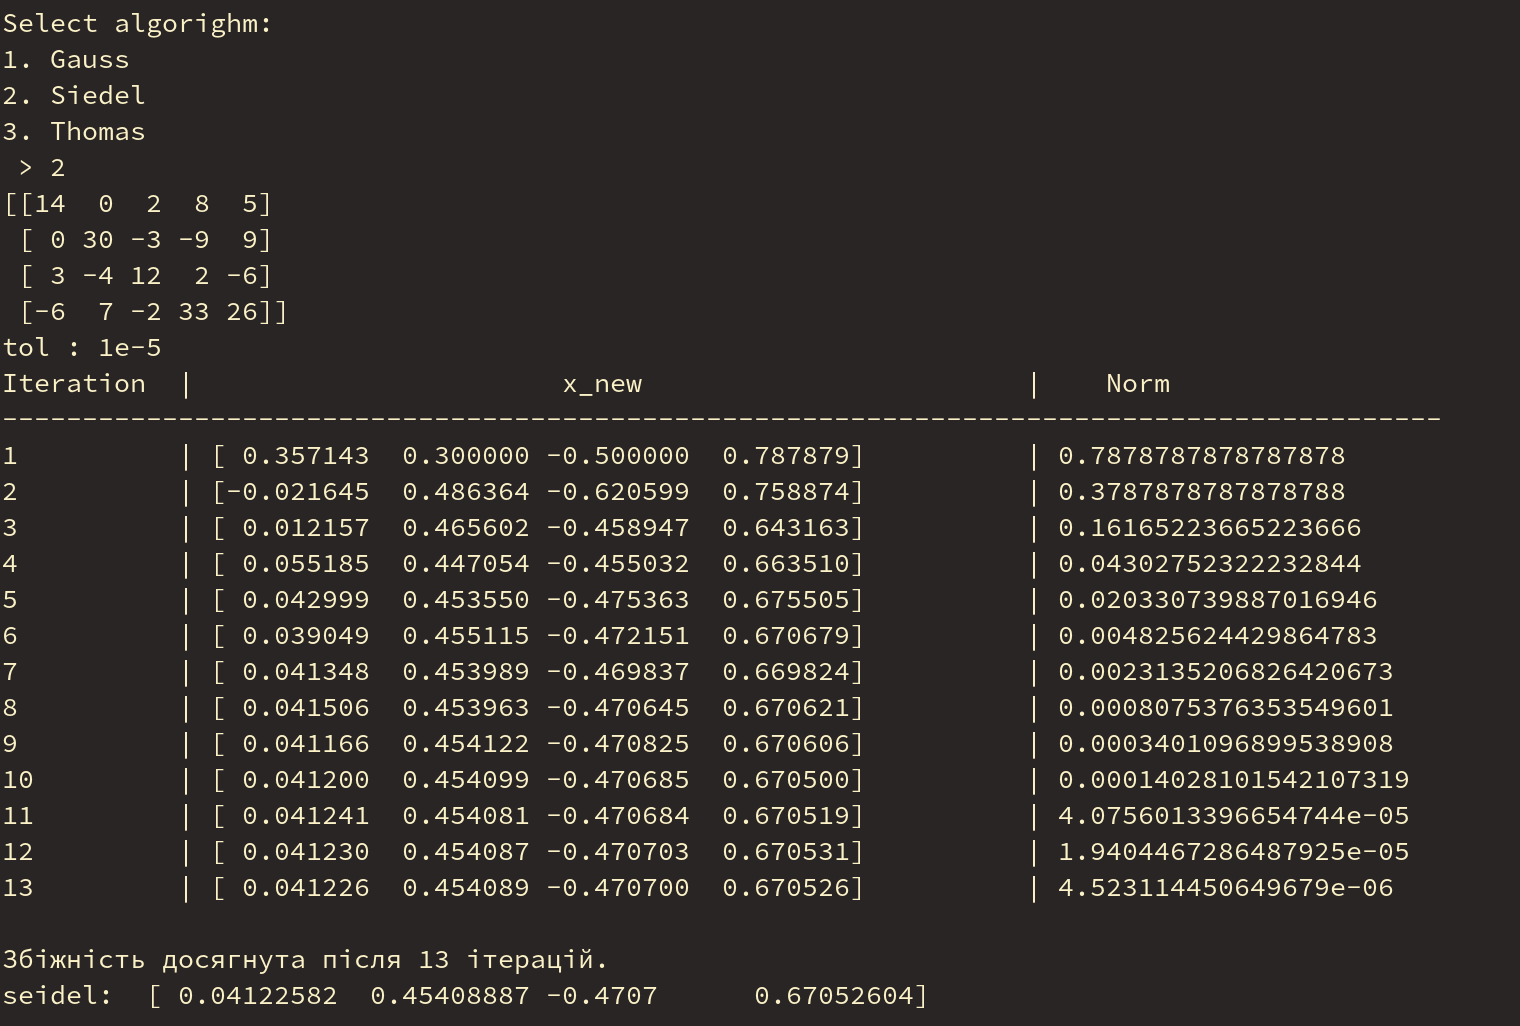
\includegraphics[width=0.8\linewidth]{seidel_result.png}
\end{figure}

Отримали відповідь ту що й методом Гауса (без урахування точності).

\newpage
\section{Висновок}

У даній лабораторній роботі були досліджені три методи розв'язку систем
лінійних рівнянь: метод Гаусса, метод Томаса та метод Зейделя. Кожен з цих
методів був реалізований на Python, і їх ефективність була перевірена на
конкретних прикладах.

1. Метод Гаусса є одним з найпоширеніших методів для розв'язку систем
рівнянь, оскільки він підходить для широкого спектра систем. Основна перевага
цього методу полягає в його універсальності, однак для великих систем він може
бути менш ефективним через складність обчислень.

2. Метод Томаса (або алгоритм прогонки) виявився найбільш ефективним для
тридіагональних матриць. Він показав себе як швидкий та економічний у
використанні обчислювальних ресурсів метод, коли система має специфічну
тридіагональну структуру.

3. Метод Зейделя є ітераційним методом, який забезпечує розв'язок за
допомогою послідовних наближень. Його основною перевагою є можливість роботи з
великими системами, але конвергенція залежить від властивостей матриці. Цей
метод може бути ефективним, коли матриця має властивість діагональної
переважності або інші спеціальні умови.

Під час виконання лабораторної роботи було проведено аналіз збіжності
ітераційного методу Зейделя, і продемонстровано, що метод може забезпечити
високу точність результатів за відносно невелику кількість ітерацій за певних
умов. Також метод Томаса продемонстрував свою ефективність для систем із
тридіагональною структурою, дозволяючи отримати розв'язок з мінімальними
витратами на обчислення.

Загалом, лабораторна робота дозволила глибше ознайомитися з різними чисельними
методами, їх перевагами та недоліками. Отримані знання та навички можуть бути
застосовані в інших задачах лінійної алгебри та обчислювальної математики,
особливо у випадках великих або спеціальних систем рівнянь.

\end{document}
